\documentclass[11pt,a4paper]{article}
%
\usepackage{titlesec}
\usepackage[utf8]{inputenc}
\usepackage[spanish]{babel}
\usepackage[backend=bibtex]{biblatex}
\decimalpoint


%----Format----%
\usepackage{bm}
\usepackage{graphicx}
\usepackage[hidelinks]{hyperref}
\usepackage[vmargin=2.5cm,hmargin=2.5cm]{geometry}
\usepackage{fancyhdr}
\pagestyle{fancy}


\setlength{\headheight}{14pt}
\rhead{Electrónica analógica}
\lhead{Ingeniería de telecomunicaciones}

\author{Antonio Cantudo} % Author name
\date{\today} % Date for the report
\usepackage{caption}
\captionsetup[table]{skip=5pt}
\usepackage{array}
\usepackage{multicol}
\usepackage{boldline}
\setlength\extrarowheight{2pt}
\usepackage{color}
\setcounter{secnumdepth}{4}
% \usepackage[framed,numbered,autolinebreaks,useliterate]{mcode}

%--Code--%
\usepackage{mathrsfs,amsmath,amsfonts,amssymb}
\makeatletter
\renewcommand\env@cases[1][l]{%
	\let\@ifnextchar\new@ifnextchar
	\left\lbrace
	\def\arraystretch{1.2}%
	\array{@{}l@{\quad}#1@{}}%
}
\makeatother

%----Diagrams----%
\usepackage{tikz}
\usepackage[siunitx]{circuitikz}
\usepackage{siunitx}
\usetikzlibrary{shapes, calc,babel,arrows,intersections}
\usepackage{pgfplots}
\pgfplotsset{compat=newest}
\usepackage{mathtools}

\begin{document}

\title{title}
\author{author}
\date{date}

\begin{titlepage}
  \begin{figure}[t]
    \centering
\includegraphics[width=0.5\textwidth]{ugrlogo}
  \end{figure}
  \begin{center}
    \textsc{ \Huge{Universidad de Granada \\}}
    \textsc{ \LARGE{Grado en ingeniería\\de telecomunicaciones\\ }}
    \textnormal{ \LARGE{Electrónica analógica\\}}
    \vspace{30mm}
    \fontsize{20mm}{7mm}\selectfont
    \textup{Práctica 1.\\Polarización de transistores.}\\
  \end{center}

  \vspace{25mm}

  \begin{minipage}[t]{0.47\textwidth}
    \textnormal{\large{\bf \\}}
    {\large }
  \end{minipage}\hfill\begin{minipage}[t]{0.47\textwidth}\raggedleft
    %\textnormal{\Large{\bf Autor\\}}
    {\Large{Pedro Javier Belmonte Miñano}\\
     \Large{Antonio Cantudo Gómez}\\
     \large{Grupo A2}}
  \end{minipage}

  \vspace{20mm}

  \centering{\Large{Curso 2019-2020 \\ 03/04/2020 }}
\end{titlepage}

\pagenumbering{gobble}

\tableofcontents

\listoffigures
\thispagestyle{plain}
\newpage
\addtocontents{toc}{~\hfill\textbf{Página}\par}
\renewcommand{\abstractname}{Objetivo}
\pagenumbering{arabic}
\captionsetup{justification=centering,margin=2cm}

	\begin{abstract}
		Durante esta práctica simularemos y analizaremos de forma teórica la polarización DC de transistores MOSFET en el circuito de la figura \ref{circuito_main}.
	\end{abstract}

	\begin{figure}[!hbt]
		\centering
		\begin{circuitikz}[american,]
			\ctikzset{tripoles/mos style/arrows}
			\def\killdepth#1{{\raisebox{0pt}[\height][0pt]{#1}}}
			\node (orig) at (0,0) {};
			\draw (0,-3) to[R, l2^=$R_{\mathrm{G_1}}$ and \SI{10}{\kilo\ohm}, n=RG1] ++(0,3) node[vcc](VCC){$V_{\mathrm{cc}}=\SI{10}{V}$} to[short, f<=$I_{\mathrm{G}_1}$] (VCC);
			\draw (0,-3) to[R, l2_=$R_{\mathrm{G_2}}$ and \SI{10}{\kilo\ohm}] ++ (0,-3) node[ground](GND){} to[short, f<=$I_{\mathrm{G}_2}$] (GND);
			\draw (0,-3) to[short] ++(1,0)   node[anchor=west,nmos](M1){};
			\draw (M1.center) node[right]{\killdepth{$M_1$}};
			\draw (M1.D) to[R, l2^=$R_{\mathrm{D_{1}}}$ and \SI{4.7}{\kilo\ohm}, n=RS1] (M1.D |- orig) node[vcc](VCC){} to[short, f<=$I_{\mathrm{D}_1}$] (VCC);
			\draw (M1.S) to[R, l2_=$R_{\mathrm{S_{1}}}$ and \SI{2.2}{\kilo\ohm}, n=RD1] (M1.S |- GND) node[ground](GND){} to[short, f<=$I_{\mathrm{S}_1}$] (GND);

			\draw (M1.S) to[short] ++(1,0) node[anchor=west, nmos](M2){};
			\draw (M2.center) node[right]{\killdepth{$M_2$}};

			\draw (M2.D) to[R, l2^=$R_{\mathrm{D_{2}}}$ and \SI{330}{\ohm}, n=RS1] (M2.D |- orig) node[vcc](VCC){} to[short, f<=$I_{\mathrm{D}_2}$] (VCC);

			\draw (M2.S) to[R, l2_=$R_{\mathrm{S_{2}}}$ and \SI{1}{\kilo\ohm}, n=RS1] (M2.S |- GND) node[ground](GND){} to[short, f<=$I_{\mathrm{S}_2}$] (GND);

		\end{circuitikz}
		\caption{Circuito de polarización}
		\label{circuito_main}
	\end{figure}

\section{Análisis teórico}

	\subsection{Fundamento teórico}
    Esta pr\'actica esta basada en los modelos te\'oricos que describen el comportamiento de un MOSFET de canal n. Estos modelos relacionan la corriente entre drenador y fuente del transistor, $I_\mathrm{DS}$, con la tensi\'on puerta fuente, $V_\mathrm{GS}$ y la tensi\'on drenador fuente, $V_\mathrm{DS}$.

    De forma general, atendiendo a la curva $V_\mathrm{DS}-I_\mathrm{DS}$, un MOSFET se puede encontrar, en uno de tres estados de polarización posibles, estado de corte, de triodo o lineal, y de saturaci\'on. Cada uno de estos estados corresponde con una de las zonas de polarización de la curva, representada en la figura \ref{zonas_mosfet}.

		El transistor se encuentra en corte siempre que el voltaje puerta fuente, $V_\mathrm{GS}$, sea menor que un determinado valor llamado tensión umbral, $V_\mathrm{T}$. Se denomina zona de corte pues la corriente que atraviesa el MOSFET, bajo esta condición, es prácticamente nula.

		La zona intermedia, a partir de la cual el MOSFET empieza a conducir, se denomina zona lineal. Decimos que un MOSFET está en estado de polarización lineal cuando se cumple $V_\mathrm{DS}< V_\mathrm{GS}-V_\mathrm{T}$ y además la tensión puerta fuente es mayor que la tensión umbral. En este tramo la curva $V_\mathrm{DS}-I_\mathrm{DS}$ se comporta de forma análoga a la curva $\Delta V-I$ de un diodo si consideramos para el mismo el modelo lineal a tramos, por lo que se la conoce como zona lineal o de triodo.

		La ultima zona de todas, la zona de saturación aparece cuando $V_\mathrm{DS}\geq V_\mathrm{GS}-V_\mathrm{T}$. En esta zona, de acuerdo con el modelo que vamos a usar, podemos aproximar el comportamiento del la curva como una recta de pendiente $\frac{k_n}{2}\left(V_{\mathrm{GS}}-V_{\mathrm{T}}\right)^2\lambda$ y de ordenada en el origen $\frac{k_n}{2}\left(V_{\mathrm{GS}}-V_{\mathrm{T}}\right)^2$. El punto donde esta recta corta al eje x se denomina tensión Early o $V_\mathrm{A}$. El hecho de que la recta tenga pendiente no nula es provocado por el efecto Early, un fenómeno que consiste en la reducción del grosor o longitud del canal de conducción formado en el MOSFET conforme aumenta la tensión drenador fuente, $V_\mathrm{DS}$. El aumento de la intesidad se debe a que la resistencia del canal es directamente proporcional a la longitud del mismo, al disminuir su longitud, disminuye por tanto su resistencia y la intensidad a través del MOSFET aumenta de acuerdo con la ley de Ohm.

    \begin{equation}
			\begin{cases}
			I_{\mathrm{DS}} = 0, & \mbox{si }V_{\mathrm{GS}}< V_{\mathrm{T}}.\\
			I_{\mathrm{DS}} = \frac{k_n}{2}\left(2\left(V_{\mathrm{GS}}-V_{\mathrm{T}}\right)V_{\mathrm{DS}}-V_{\mathrm{DS}}^2\right), & \mbox{si } V_{\mathrm{GS}}\geq V_{\mathrm{T}} \mbox{ y }V_{\mathrm{DS}}\leq V_{\mathrm{GS}}-V_{\mathrm{T}}.\\
			I_{\mathrm{DS}} = \frac{k_n}{2}\left(V_{\mathrm{GS}}-V_{\mathrm{T}}\right)^2\left(1+\lambda V_{\mathrm{DS}}\right), & \mbox{si } V_{\mathrm{GS}}\geq V_{\mathrm{T}} \mbox{ y } V_{\mathrm{GS}}-V_{\mathrm{T}}< V_{\mathrm{DS}}.
			\end{cases}
			\label{eq_mosfet}
		\end{equation}

		Esta es la curva representada para los modelos estudiados en clase, sin embargo, para los transistores reales, estas ecuaciones, debido a las aproximaciones e idealizaciones supuestas para su cálculo, no se cumplen con exactitud. En particular, para la curva $V_\mathrm{DS}-I_\mathrm{DS}$ los MOSFET reales alcanzan, para un cierto valor de $V_\mathrm{DS}$ un máximo valor de $I_\mathrm{DS}$ a partir del cual, aumentos de la tensión drenador fuente producen decrementos en la corriente $I_\mathrm{DS}$.

    \begin{figure}[!hbt]
      \centering
      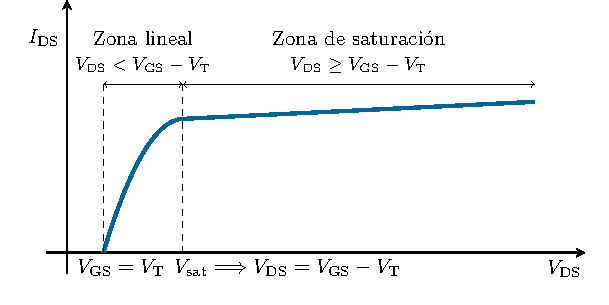
\includegraphics[width=0.8\columnwidth]{figuras/mosfet-curva}
      \caption{Zonas de polarización de un MOSFET}
      \label{zonas_mosfet}
    \end{figure}



	\subsection{Cálculo teórico de la polarización.}



		Considerando nula la corriente de puerta en los MOSFETs, y usando las ecuaciones \ref{eq_mosfet}, procedemos a estudiar de forma teórica el circuito de la figura \ref{circuito_main}, primero obtendremos los valores de tensión y corriente de los terminales del transistor M1, para ello supondremos que trabaja en estado de saturación.

		\begin{align*}
			&\hspace{2pt}I_1 = I_2 \\
			\frac{V_1 - V_{\mathrm{G}_1}}{R_1} = \frac{V_{\mathrm{G}_1}}{R_2} &\xRightarrow{R_1 = R_2} V_{\mathrm{G}_1} = \frac{V_1}{2} = \SI{5}{\volt} \\
			&\hspace{2pt}I_3 = I_2 \\
			\frac{V_1 - V_{\mathrm{D}_1}}{R_3} = \frac{K_n}{2}(V_{\mathrm{GS}_1} - V_{\mathrm{T}})^2 &\xRightarrow{\hspace{27pt}} V_{\mathrm{D}_1} = V_1 - \frac{K_n}{2}R_3(V_{\mathrm{G}_1}-V_{\mathrm{S}_1}-V_{\mathrm{T}})^2 \\
			&\hspace{2pt}I_4 = I_{\mathrm{D}_1} \\
			\frac{V_{\mathrm{S}_1}}{R_4} = \frac{K_n}{2}(V_{\mathrm{GS}_1} - V_{\mathrm{T}})^2 &\xRightarrow{\hspace{27pt}} 12.1V_{\mathrm{S}_1}^2 - 77.23V_{\mathrm{S}_1} + 120.03 = 0
		\end{align*}

		Obtenemos dos valores de $V_{\mathrm{S}_1}$ y de $V_{\mathrm{D}_1}$, que cumplen las condiciones de las zonas de saturación, es decir, $V_{\mathrm{GS}} \geq V_{\mathrm{T}}$ y $V_{\mathrm{DS}} \geq V_{\mathrm{GS}} -  V_{\mathrm{T}}$.
		\begin{align*}
			\hspace{-39pt}V_{\mathrm{S}_1} =
			\begin{cases}
				\SI{3,71}{\volt} \\
				\SI{2,68}{\volt} \checkmark
			\end{cases} &\xRightarrow{\hspace{27pt}}
			V_{\mathrm{D}_1} =
			\begin{cases}
				\SI{2,01}{\volt} \\
				\SI{4,22}{\volt} \checkmark
			\end{cases} \\
			&\hspace{-4pt}I_{\mathrm{D}_1} = \SI{1,23}{\milli\ampere}
		\end{align*}
		\begin{equation*}
			\begin{cases}
				V_\mathrm{GS} &= \SI{2.32}{\volt} \geq \SI{1.85}{\volt} =  V_\mathrm{T}\\
				V_\mathrm{DS} &= \SI{1.54}{\volt} \geq \SI{2.32}{\volt}-\SI{1.85}{\volt} = V_\mathrm{GS} - V_\mathrm{T}
			\end{cases}
		\end{equation*}

		De forma análoga realizaremos los cálculos para el transistor M2. Obteniendo dos valores de tensión, $V_\mathrm{S_2}$ y $V_\mathrm{D2}$ que cumplen las condiciones de saturación.

		\begin{align*}
			&\hspace{2pt}I_{\mathrm{S}} = I_{\mathrm{D}_2} \\
			\frac{V_1 - V_{\mathrm{D}_2}}{R_5} = \frac{K_n}{2}(V_{\mathrm{GS}_2} - V_{\mathrm{T}})^2 &\xRightarrow{\hspace{27pt}} V_{\mathrm{D}_2} = V_1 - \frac{K_n}{2}R_3(V_{\mathrm{G}_2}-V_{\mathrm{S}_2}-V_{\mathrm{T}})^2 \\
			&\hspace{2pt}I_6 = I_{\mathrm{D}_2} \\
			\frac{V_{\mathrm{S}_2}}{R_6} = \frac{K_n}{2}(V_{\mathrm{GS}_2} - V_{\mathrm{T}})^2 &\xRightarrow{\hspace{27pt}} 5.5V_{\mathrm{S}_2}^2 - 10.17V_{\mathrm{S}_2} + 3.83 = 0 \\
			V_{\mathrm{S}_2} =
			\begin{cases}
				\SI{1.32}{\volt} \\
				\SI{0.53}{\volt} \checkmark
			\end{cases} &\xRightarrow{\hspace{27pt}}
			V_{\mathrm{D}_2} =
			\begin{cases}
				\SI{9.56}{\volt} \\
				\SI{9.83}{\volt} \checkmark
			\end{cases} \\
			&\hspace{-4pt}I_{\mathrm{D}_2} = \SI{0.53}{\milli\ampere}
		\end{align*}
		\begin{equation*}
			\begin{cases}
				V_\mathrm{GS} &= \SI{2.15}{\volt} \geq \SI{1.85}{\volt} =  V_\mathrm{T}\\
				V_\mathrm{DS} &= \SI{9.30}{\volt} \geq \SI{2.15}{\volt}-\SI{1.85}{\volt} = V_\mathrm{GS} - V_\mathrm{T}
			\end{cases} \\
		\end{equation*}

		Como vemos los dos transistores trabajan en modo de saturación. A continuación se muestran los resultados finales:

		\begin{table}[!hbt]
			\centering
			\caption{Resultados obtenidos en el análisis teórico}
			\begin{tabular}{c | c c}
				& $\mathrm{M}_1$ & $\mathrm{M}_2$ \\
				\hline\hline
				$V_\mathrm{G}$(V) & 5,00 & 2.68 \\
				% \hline
				$V_\mathrm{D}$(V) & 4.22 & 9.83 \\
				% \hline
				$V_\mathrm{S}$(V) & 2.68 & 0.53 \\
				% \hline
				$I_{\mathrm{DS}}$(mA) & 1.22 & 0.53
			\end{tabular}
			\label{tabla_resultadosanalisis}
		\end{table}


		\section{Simulación}

		Hemos simulado el comportamiento del circuito mediante el software LtSpice. En la figura \ref{simulacion_esquematico} podemos observar una captura del esquemático simulado. Hemos considerado, puesto que no conocemos ni hemos podido obtener experimentalmente el valor de la tensión Early, despreciable el efecto Early, estableciendo a cero el parámetro lambda, $\lambda$, del transistor NMOS en Spice. Además de $\lambda$ hemos configurado la tensión umbral, $V_\mathrm{T}$ y el parámetro de transconductancia, $k_n$. Puesto que únicamente queremos estudiar el comportamiento del circuito en DC y para un único valor de la fuente de voltaje, hemos simulado el circuito en modo \emph{Operating point}, a fin de obtener las corrientes y tensiones en cada nudo y malla del mismo.

		\begin{figure}[!hbt]
			\centering
			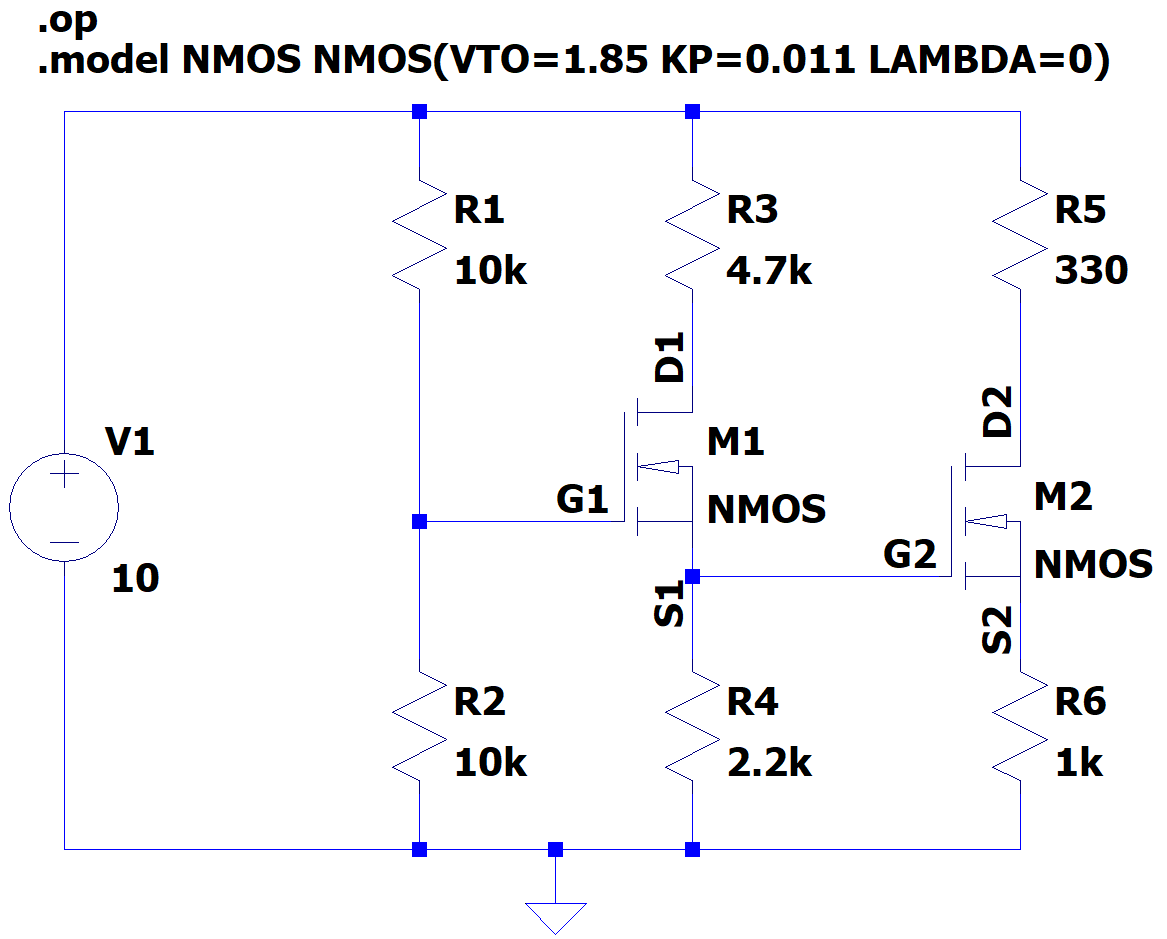
\includegraphics[width=0.5\columnwidth]{figuras/simulacion_esquematico}
			\caption{Captura del esquemático simulado en LtSpice}
			\label{simulacion_esquematico}
		\end{figure}

		\newpage
		Los resultados obtenidos de la simulación se recogen en la siguiente tabla.
		\begin{table}[!hbt]
			\centering
			\caption{Resultados de la simulación en LtSpice}
			\begin{tabular}{c | c c}
				& $\mathrm{M}_1$ & $\mathrm{M}_2$ \\
				\hline\hline
				$V_\mathrm{G}$(V) & 5 & 2.67 \\
				% \hline
				$V_\mathrm{D}$(V) & 4.28 & 9.83 \\
				% \hline
				$V_\mathrm{S}$(V) & 2.68 & 0.5215 \\
				% \hline
				$I_{\mathrm{DS}}$(mA) & 1.21 & 0.52 \\
				\hline\hline
			\end{tabular}
			\label{tabla_resultadossim}
		\end{table}

		Como podemos comprobar los resultados de la simulación se corresponden de forma casi exacta con los obtenidos en el análisis teórico, cuadro \ref{tabla_resultadosanalisis}, por lo que podemos concluir que los cálculos realizados son correctos y ambos transistores se encuentran polarizados en saturación.

\section{Conclusión}

	Hemos comprobado que los dos transistores se encontraban en régimen de saturación y que el modelado simplificado del transistor MOSFET estudiado en clase se aproxima bastante bien a los modelos complejos implementados en el software LtSpice para este tipo de circuitos.

\end{document}
